\section*{\fs{12}Zapytanie do jednej tablicy}
\subsection*{\fs{12} Data zatrudnienia Trevor Sanford }
\par{
\fs{12}


\listsinglespacing{
\fs{12}
\begin{lstlisting}[frame=single,language=SQL,]
Select data_zatrudnienia as Zatrudniony
from  Pracownicy
where imie='Trevor' and nazwisko='Sanford'

\end{lstlisting}
\begin{figure}[h!]
    \centering
   \scalebox{.85}{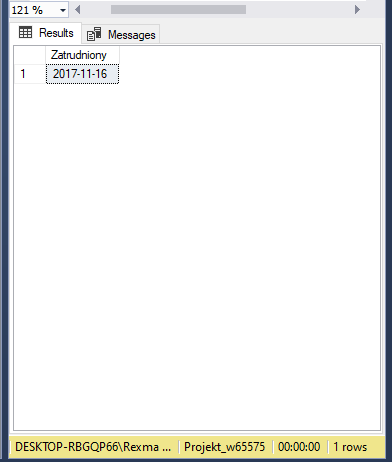
\includegraphics{Images/Zadanie3/P1/Z1a.png}}
    \caption{Wynik Zapytania}
    \label{fig:my_label}
\end{figure}

}
\begin{figure}[h!]
    \centering
   \scalebox{.70}{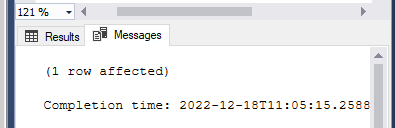
\includegraphics{Images/Zadanie3/P1/Z1b.png}}
    \caption{Wynik Zapytania}
    \label{fig:my_label}
\end{figure}
}
\newpage

\subsection*{\fs{12} Pracownicy zarabiajacy ponad 10000 w kolejnosci alfabetyczne }
\listsinglespacing{
\fs{12}
\begin{lstlisting}[frame=single,language=SQL,]
Select imie,nazwisko
from  Pracownicy
where wypłata>=10000
order by nazwisko

\end{lstlisting}
\begin{figure}[h!]
    \centering
   \scalebox{.85}{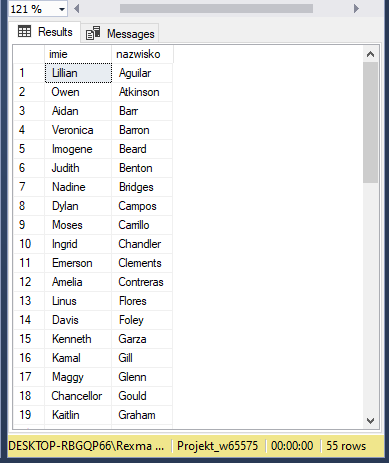
\includegraphics{Images/Zadanie3/P1/Z2a.png}}
    \caption{Wynik Zapytania}
    \label{fig:my_label}
\end{figure}

}

\begin{figure}[h!]
    \centering
   \scalebox{.70}{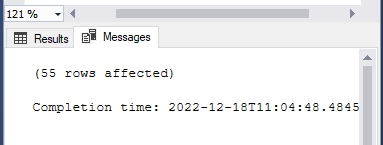
\includegraphics{Images/Zadanie3/P1/Z2b.png}}
    \caption{Wynik Zapytania}
    \label{fig:my_label}
\end{figure}


\newpage
\subsection*{\fs{12} Nr telefonu do  Zorana	Deroche}
\listsinglespacing{
\fs{12}
\begin{lstlisting}[frame=single,language=SQL,]
Select nr_telefonu as Kontakt
from  Pacjent
where imie='Zorana' and nazwisko='Deroche'

\end{lstlisting}
\begin{figure}[h!]
    \centering
   \scalebox{.85}{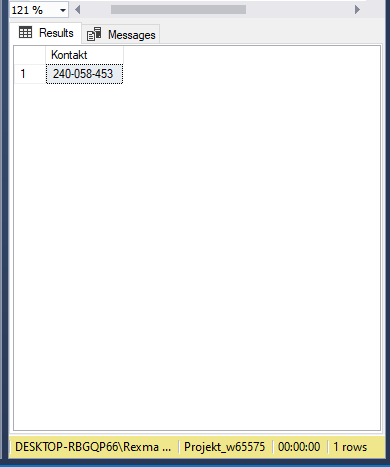
\includegraphics{Images/Zadanie3/P1/Z3a.png}}
    \caption{Wynik Zapytania}
    \label{fig:my_label}
\end{figure}

}
\begin{figure}[h!]
    \centering
   \scalebox{.70}{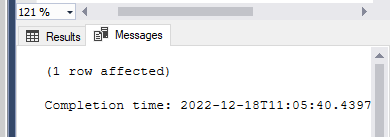
\includegraphics{Images/Zadanie3/P1/Z3b.png}}
    \caption{Wynik Zapytania}
    \label{fig:my_label}
\end{figure}

\newpage

\subsection*{\fs{12} Wypisanie zarobków}
\listsinglespacing{
\fs{12}
\begin{lstlisting}[frame=single,language=SQL,]
Select imie,nazwisko, 
CASE
	When Wypłata<5000 THEN 'Zarabia mało'
	WHEN Wypłata>5000 THEN 'Zarabia średnio'
	WHEN Wypłata>10000 THEN 'Zarabia dużo'
END
as [Ile zarabia]
from Pracownicy

\end{lstlisting}
}
\begin{figure}[h!]
    \centering
   \scalebox{.85}{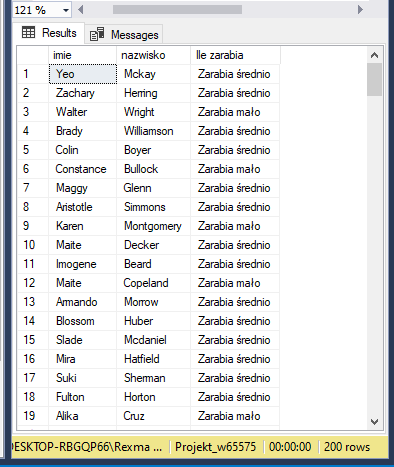
\includegraphics{Images/Zadanie3/P1/Z4a.png}}
    \caption{Wynik Zapytania}
    \label{fig:my_label}
\end{figure}
\begin{figure}[h!]
    \centering
   \scalebox{.70}{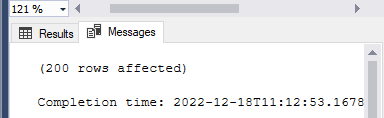
\includegraphics{Images/Zadanie3/P1/Z4b.png}}
    \caption{Wynik Zapytania}
    \label{fig:my_label}
\end{figure}\newpage

\subsection*{\fs{12} Wygnerowanie emailów dla pracowników}
\listsinglespacing{
\fs{12}
\begin{lstlisting}[frame=single,language=SQL,]
Select imie,nazwisko,
CONCAT(lower(imie),'-',LOWER(nazwisko),'@hospital.com') as Email 
from Pracownicy

\end{lstlisting}
}
\begin{figure}[h!]
    \centering
   \scalebox{.85}{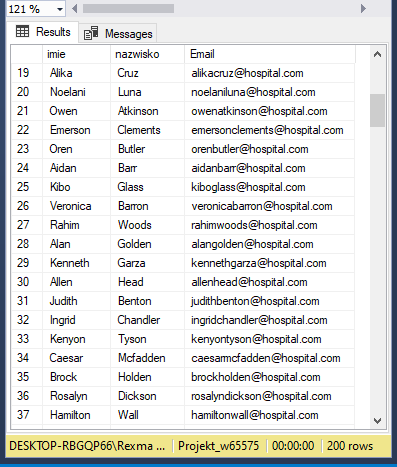
\includegraphics{Images/Zadanie3/P1/Z5a.png}}
    \caption{Wynik Zapytania}
    \label{fig:my_label}
\end{figure}
\begin{figure}[h!]
    \centering
   \scalebox{.70}{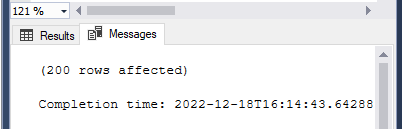
\includegraphics{Images/Zadanie3/P1/Z5b.png}}
    \caption{Wynik Zapytania}
    \label{fig:my_label}
\end{figure}\newpage
